\documentclass[a4paper, 12pt]{article}
\usepackage[usenames,dvipsnames,svgnames,table]{xcolor}
\usepackage[T1]{fontenc}
\usepackage{times}
\usepackage[utf8]{inputenc}
\usepackage{wallpaper}
\usepackage[absolute]{textpos}
\usepackage[top=2cm, bottom=2.5cm, left=3cm, right=3cm]{geometry}
\usepackage{sectsty}
\sectionfont{\fontsize{14}{15}\selectfont}
\subsectionfont{\fontsize{12}{15}\selectfont}
\subsubsectionfont{\fontsize{12}{15}\selectfont}
\usepackage{algorithm}
\usepackage[noend]{algpseudocode}
\usepackage{listings}
\usepackage{amsmath}
\usepackage{amsfonts}
\usepackage[hang]{footmisc}

\definecolor{MyDarkGreen}{rgb}{0.0,0.4,0.0} % This is the color used for comments
\lstloadlanguages{AVR}%
\lstset{language=AVR, % AVR 8-bit Assembler
        basicstyle=\tiny,
        literate={å}{{\ra}}1
                 {ä}{{\"a}}1
                 {ö}{{\"o}}1,
        keywordstyle=\color{Blue}\bf, % Instructions in blue, bold
        keywordstyle=[2]\color{Orange}, % Registers and ports in orange
        keywordstyle=[3]\color{Purple}, % Directives in purple
        commentstyle=\color{MyDarkGreen},
        tabsize=4, % 5 spaces per tab
        numbers=left, % Line numbers on left
        firstnumber=1, % Line numbers start with line 1
        numberstyle=\tiny\color{Blue}, % Line numbers are blue and small
        stepnumber=1 % Line numbers go in steps of 5
}

% Creates a new command to include an asm script,
% the first parameter is the filename of the program (without .asm),
% the second parameter is the caption
\newcommand{\avrasm}[2]{
\begin{itemize}
\item[]\lstinputlisting[caption=#2,label=#1]{#1}
\end{itemize}
}

\newsavebox{\mybox}
\newlength{\mydepth}
\newlength{\myheight}
\newenvironment{sidebar}
{\begin{lrbox}{\mybox}\begin{minipage}{\textwidth}}
{\end{minipage}\end{lrbox}
 \settodepth{\mydepth}{\usebox{\mybox}}
 \settoheight{\myheight}{\usebox{\mybox}}
 \addtolength{\myheight}{\mydepth}
 \noindent\makebox[0pt]{\hspace{-20pt}\rule[-\mydepth]{1pt}{\myheight}}
 \usebox{\mybox}}

\newcommand\BackgroundPic{
    \put(-2,-3){
    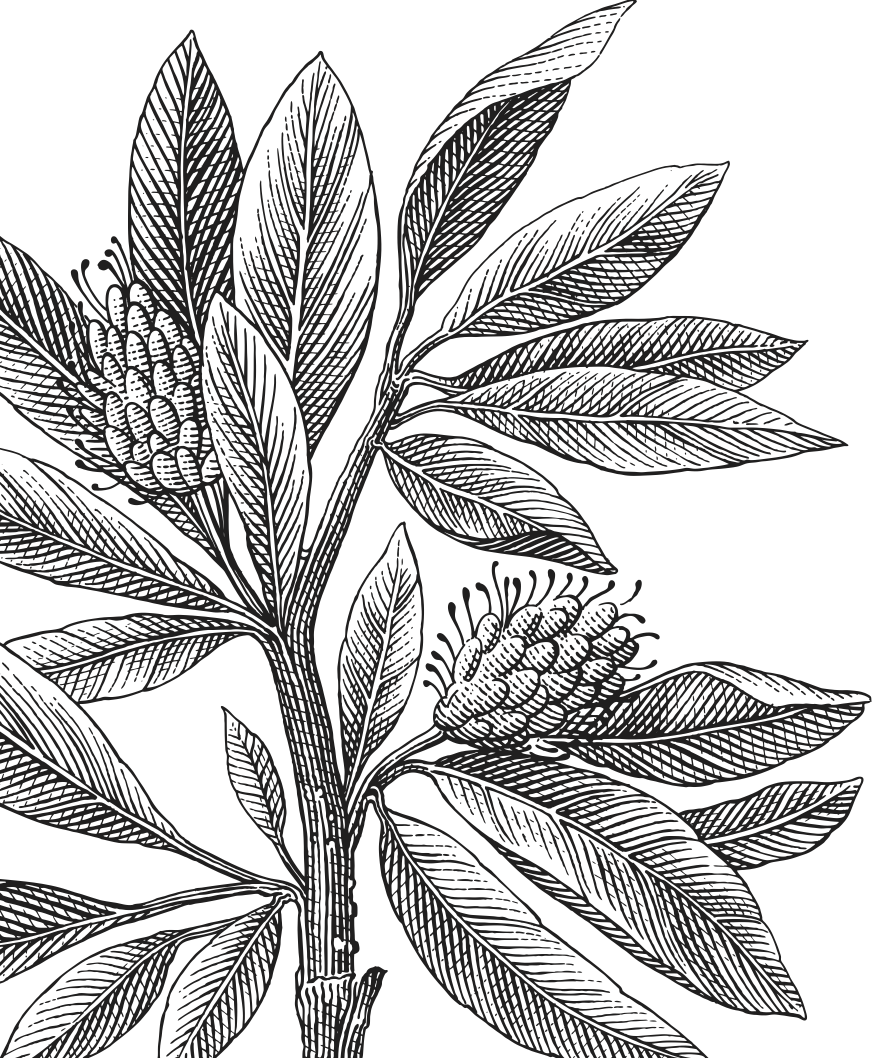
\includegraphics[keepaspectratio,scale=0.3]{lnu_etch.png} 
    }
}
\newcommand\BackgroundPicLogo{
    \put(30,740){
	
\includegraphics[keepaspectratio,scale=0.10]{logo.png}     
    }
}

\title{	
\vspace{-8cm}
\begin{sidebar}
    \vspace{5cm}
    \normalfont \normalsize
    \Huge Report \\
    \vspace{-1.3cm}
\end{sidebar}
\vspace{3cm}
\begin{flushleft}
    \huge Laboratory 1\\  
\end{flushleft}
\null
\vfill
\begin{textblock}{6}(10,13)
\begin{flushright}
\begin{minipage}{\textwidth}
\begin{flushleft} \large
	\emph{Author:} Caroline Nilsson \\ Daniel Alm Grundström \\
	%\emph{Handledare:} \\ 
	\emph{Term:} HT 2017\\ 
	\emph{Course:} 1DT301 - Computer Technology I\\
\end{flushleft}
\end{minipage}
\end{flushright}
\end{textblock}
}
\date{\today} 

\begin{document}

\pagenumbering{gobble}
\newgeometry{left=5cm}
\AddToShipoutPicture*{\BackgroundPic}
\AddToShipoutPicture*{\BackgroundPicLogo}
\maketitle
\restoregeometry
\clearpage

\pagenumbering{gobble}

\tableofcontents
\newpage
\pagenumbering{arabic}

\section{Introduction}
In the process of working with the laboratory assignments we started by doing research about the AVR Assembly language and the STK600 in order to better understand how to solve the different assignments.
In each assignment we first created a pseudocode solution which we converted to flowchart diagrams, then it was rather simple to convert this into Assembly code. Common for all assignments is also that we have been using the simulations to confirm that the program is working and completing the correct tasks. 


\newpage

\section{Assignment 1 - Light LED2}
In the first assignment we were to write an Assembly program that lights up \texttt{LED2} (which is the third light counting from the right).


\subsection{Pseudo code}
\begin{algorithm}
\begin{algorithmic}
\Procedure{Pseudocode}{}
\State{$PortB = output$}
\State{$Led2\ bitstring \rightarrow PortB$}
\EndProcedure
\caption{Light LED2}
\label{assign1.pseudo}
\end{algorithmic}
\end{algorithm}

\subsection{Flowchart}
\begin{figure}[h]
\centering
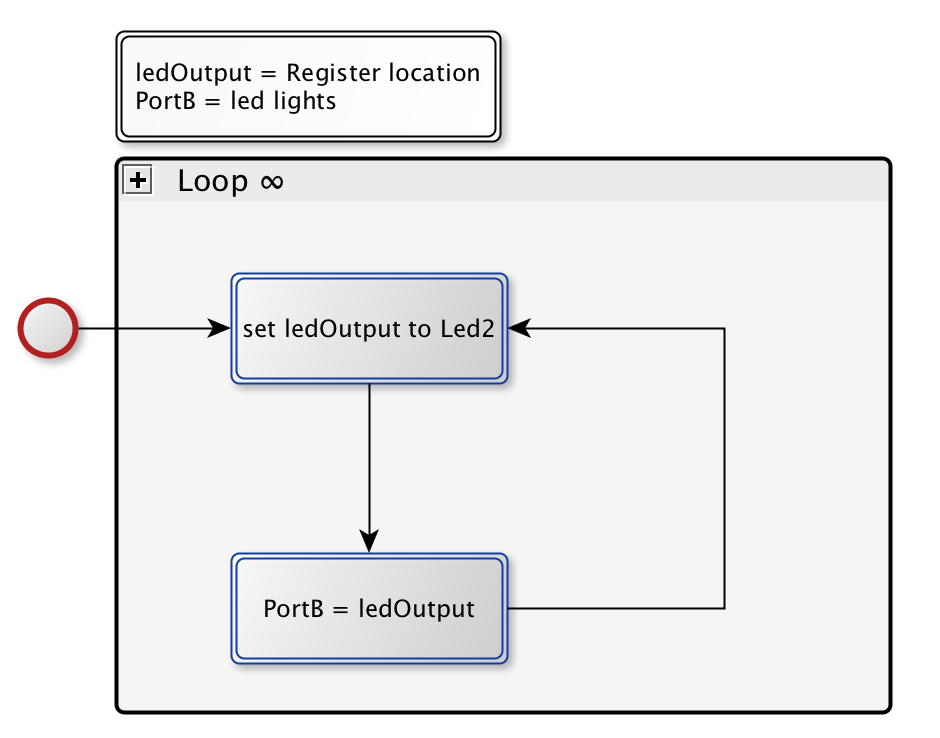
\includegraphics[scale=0.5]{Flowchart_pics/assignment1_pic.png} 
\caption{Flowchart}
\label{assign1.flow}
\end{figure}

\subsection{Method}
The pseudocode (see algorithm \ref{assign1.pseudo}) and the flowchart (see figure \ref{assign1.flow}) shows that we first set \texttt{PORTB} as an output port. To light up \texttt{LED2} we then only need to write a value to the bit on \texttt{PORTB} that corresponds to \texttt{LED2}. 

We started with the assumption that all bits in \texttt{PORTB} would be zero when the LEDs where turned off and as such wrote a 1 to the third least significant bit to light up \texttt{LED2}. When we tested the program on the hardware however, all LEDs except \texttt{LED2} was turned on. If we understood this correctly, this was due to the pull-up resistor being activated on \texttt{PORTB} which made the LEDs light when their bit was 0 (as opposed to 1) on \texttt{PORTB}. We fixed this by simply inverting the value we wrote to \texttt{PORTB} (${1111\ 1011}_2$ instead of ${0000\ 0100}_2$).

The minimal number of lines required to write this program we think are 4 (unless there is some obscure trick). 2 lines are required to set the LED port as output: 1) write a value to a register and 2) write that value to the data direction register, and 2 lines for turning on the LED: 3) write the LED state to a register and 4) write the LED state to the output port. One could try to write the program in 3 lines, by reusing the value written to the data direction register when writing to the output port. But in this case the LED will not turn on because of the pull-up resistor will require that a zero is written to the bit corresponding to the LED that we want to light.


\newpage
\subsection{Assembly Program}
\avrasm{../src/a1.asm}{}
\newpage

\section{Assignment 2 - Switch light corresponding LED}
In the second assignment we were to write a program that waits for a switch
to be pressed and then lights up the corresponding LED. For example if switch 3
is pressed LED 3 should light up. The way we interpreted the assignment was
that the LED should stay on for as long as the switch is pressed and turn off
when the switch is released.


\subsection{Pseudo code}
\begin{algorithm}
\begin{algorithmic}
\Procedure{Pseudocode}{}
\State{$PortB = output$}
\State{$PortC = input$}
\Repeat
\State{$PortC\ value \rightarrow switchState$} \Comment{$switchState = register\ location$}
\State{$switchState \rightarrow PortB$}
\Until{$\infty$}
\EndProcedure
\caption{Switches pressed lights corresponding LED}
\label{assign2.pseudo}
\end{algorithmic}
\end{algorithm}

\subsection{Flowchart}
\begin{figure}[h]
\centering
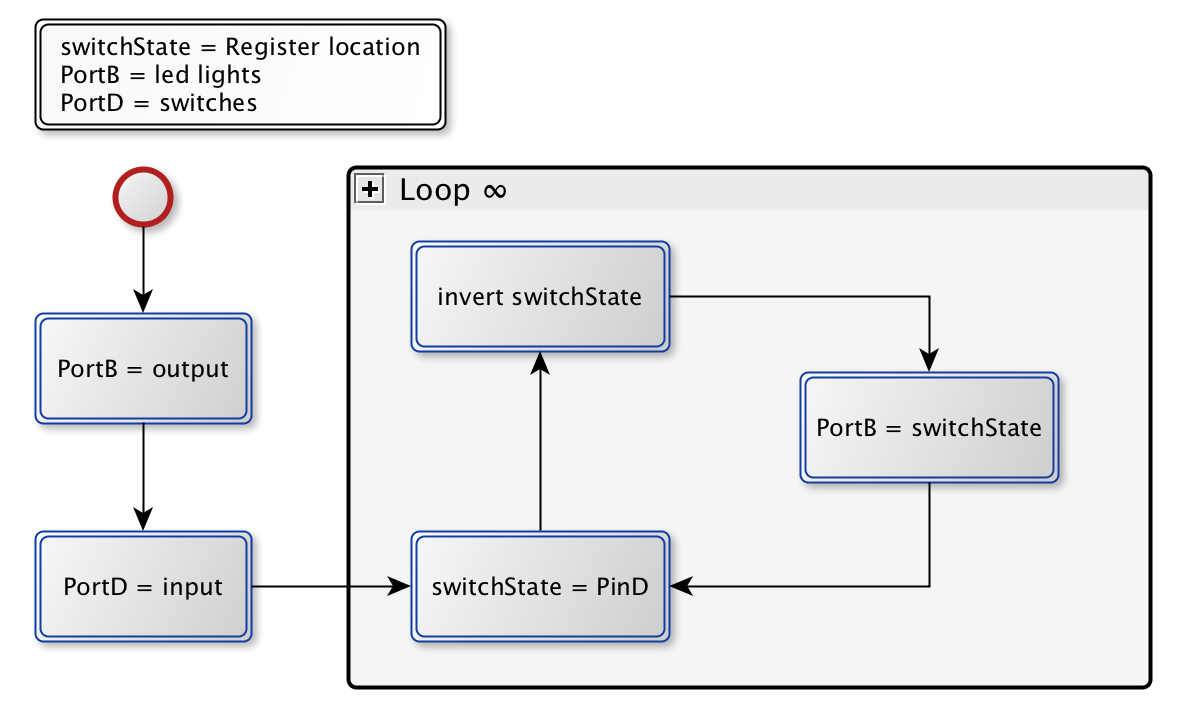
\includegraphics[scale=0.5]{Flowchart_pics/assignment2_pic.png} 
\caption{Basic flow in order to read switches and light corresponding LED}
\label{assign2.flow}
\end{figure}

\subsection{Method}
We figured the simplest way to solve this problem was to redirect the input from the switches to the LEDs repeateadly in a loop. We start by setting \texttt{PORTB} as output and \texttt{PORTC} as input. Then, in an infinite loop, we read the value of the pins on \texttt{PORTC} to a register and output the value of that register to \texttt{PORTB}.

\newpage

\subsection{Assembly Program}
\avrasm{../src/a2.asm}{}
\newpage

\section{Assignment 3 - Switch 5 lights LED0}
In the third assignment we were to write an Assembly program that turns on \texttt{LED0} when the switch \texttt{SW5} is pressed. Nothing should happen when the other switches are pressed. We assumed that the way the program should work is that the LED would stay lit for as long as \texttt{SW5} was pressed down and turn off when the switch was released.


\subsection{Pseudo code}
\begin{algorithm}
\begin{algorithmic}
\Procedure{Pseudocode}{}
\State{$PortB = output$}
\State{$PortC = input$}
\Repeat
\State{$reset\ ledState$} \Comment{$ledState = register\ location$}
\If{$Switch5\ is\ pressed$}
\State{$ledState = LED0\ bit\ string$}
\EndIf
\State{$ledState \rightarrow PortB$}
\Until{$\infty$}
\EndProcedure
\caption{Light LED0 when switch5 is pressed}
\label{assign2.pseudo}
\end{algorithmic}
\end{algorithm}

\subsection{Flowchart}
\begin{figure}[h]
\centering
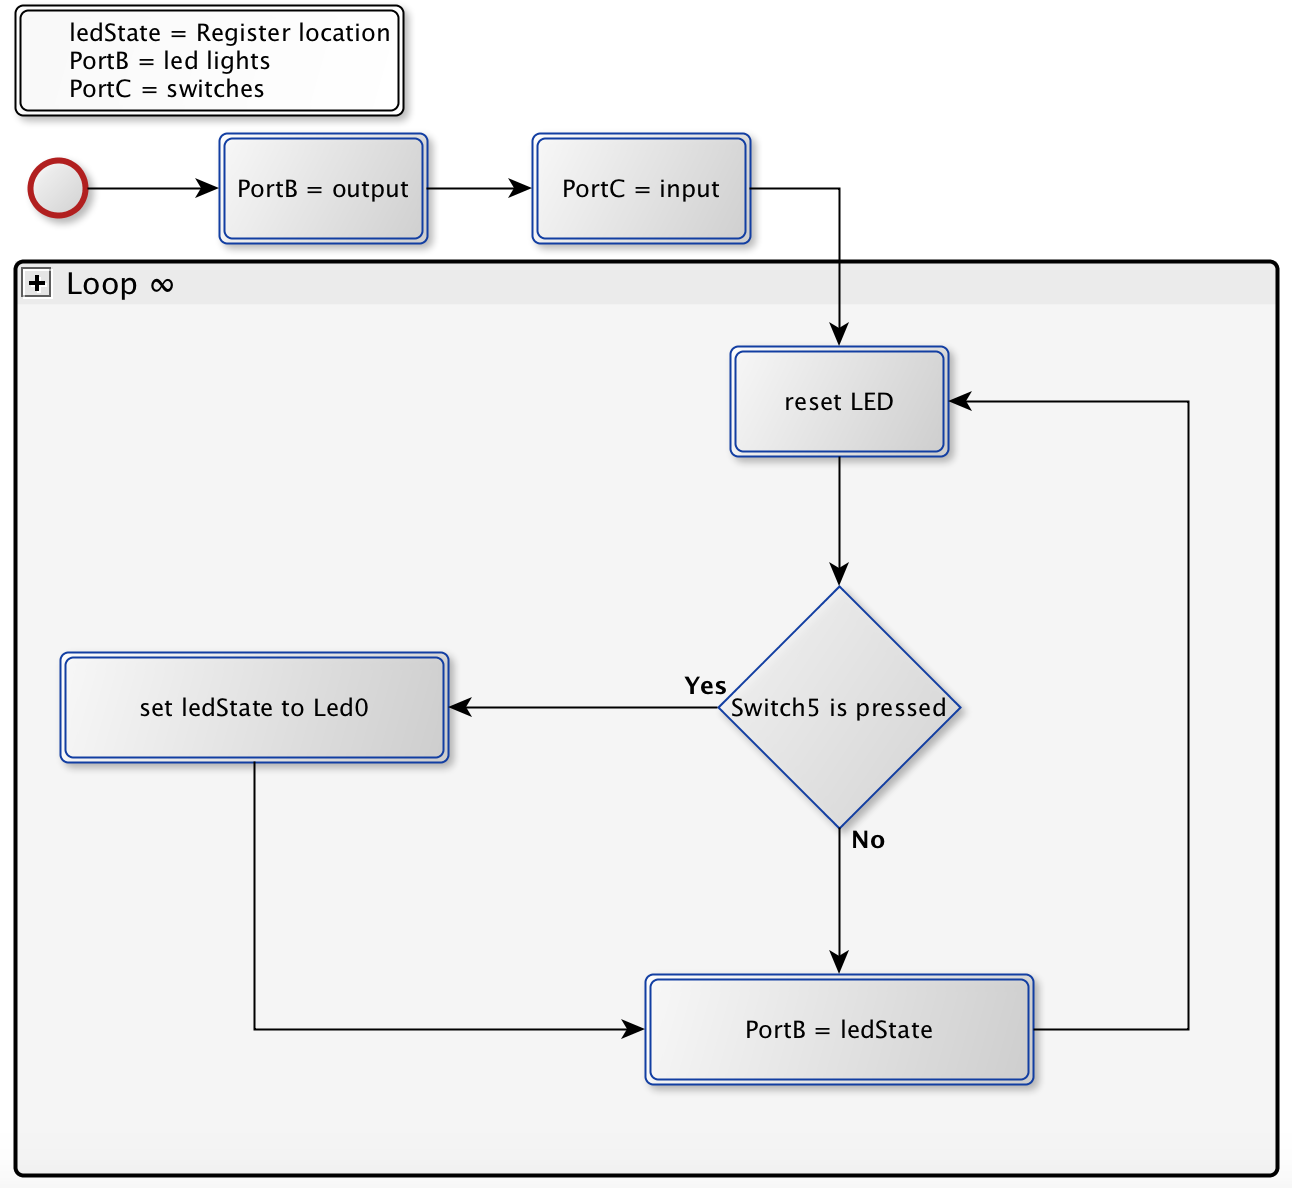
\includegraphics[scale=0.5]{Flowchart_pics/assignment3_pic.png} 
\caption{Flowchart}
\label{}
\end{figure}

\subsection{Method}
As with the previous assignment, we figured the first thing that needed to be done was to set the LED port, \texttt{PORTB}, as output and the switch port, \texttt{PORTC}, as input. In a loop, we then reset the value to write to the leds before checking if \texttt{SW5} is pressed down. If the switch is pressed down we clear the least significant bit in the LED output value to indicate that we want \texttt{LED0} to turn on before writing the value out to the LEDs.

When testing on hardware we needed to adjust the code for the pull-up resistors on the LEDs to get it to work.

\newpage

\subsection{Assembly Program}
\avrasm{../src/a3.asm}{}
\newpage

\section{Assignment 4 - Using the AVR simulator}
For this assignment, we were to take the program we wrote for the previous assignment, that lights \texttt{LED0} when \texttt{SW5} is pressed down, and run it in the AVR simulator that is included in Atmel Studio. 


\subsection{Method}
We used the AVR simulator included with \emph{Atmel Studio 6} to run the program. First, we needed to setup the debugger to run the program on the simulator which is done by selecting "Simulator" in \emph{Project} $\rightarrow$ \emph{Properties} $\rightarrow$ \emph{Tool}. To start stepping through the program we then clicked \emph{Debug} $\rightarrow$ \emph{Start debugging and break}. To be able to see what happens in the simulator as the program runs, we opened the \emph{Processor Status} and \emph{I/O} windows by clicking on their respective icons. Finally, because values from the pins on the switches have a default value of 1 we needed to set all the bits to the right of \emph{PINC}, which we did by selecting \emph{I/O Port (PORTC)} in the I/O window and filling in the bits by PINC by clicking on them.

We then started stepping through the program. The first few lines sets \texttt{PORTB} as output (line 42-43) and \texttt{PORTC} to input (line 46-47) and this can be seen in the simulator by keeping an eye on \emph{PORTB $\rightarrow$ DDRB}, which bits are set to all 1, and \emph{PORTC $\rightarrow$ DDRC}, which are set to all 0, as the debugger executes the instructions. When the debugger executes line 50, which sets all bits in the register 17, we can see this in the Processor Status window. We tested that the instruction on line 53, which checks if \texttt{SW5} is pressed down, works by manually clearing bit 5 on PINC through the I/O window. The instruction that gets executed if this is true, can be seen in the simulator in that register 17 changes value from \texttt{0xFF} to \texttt{0xFE}. The result of line 56, which writes the value of register 17 to \texttt{PORTB}, can be seen by clicking on PORTB in the I/O window where the bits next to PORTB and PINB are updated accordingly. We could also see that the \emph{Program Counter} value in the Processor Status window gets updated when the final line \texttt{rcall jump} gets executed.
\newpage

\section{Assignment 5 - Waterfall}

\subsection{Assignment description}
The fifth assignment was to write an Assembly program that outputs a ring counter to the LEDs. Between each value in the counter, there should be a delay of approximately $0.5$ seconds. Since the delay should be a subroutine in the program, the stack pointer \texttt{SP} needs to be initialized as instructed in the description of the assignment.


\subsection{Pseudo code}
\begin{algorithm}
\begin{algorithmic}
\Procedure{Pseudocode}{}
\State{$Initialize\ stack\ pointer$}
\State{$PortB = output$}
\State{$Initialize\ ledState$} \Comment{$ledState = register\ location$}
\Repeat
\State{$ledState \rightarrow PortB$}
\State{$Delay$}
\State{$rotate\ ledState\ to\ left$}
\Until{$\infty$}
\EndProcedure
\caption{Waterfall simulation using LEDs}
\label{}
\end{algorithmic}
\end{algorithm}

\subsection{Flowchart}
\begin{figure}[h]
\centering
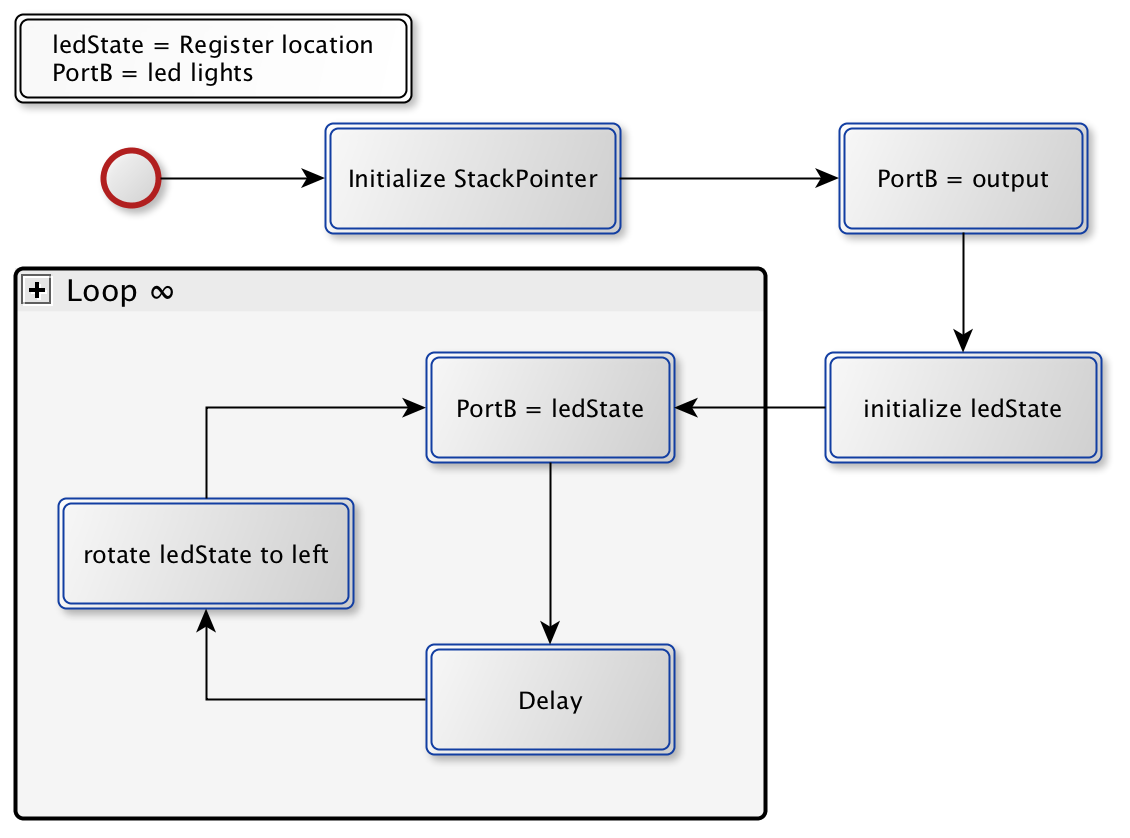
\includegraphics[scale=0.5]{Flowchart_pics/assignment5_pic.png} 
\caption{Flowchart}
\label{}
\end{figure}

\newpage
\subsection{Method}
The first thing we needed to do, as described above, was to initialize the stack pointer. This is done by setting \texttt{SP} to the end of SRAM (\texttt{RAMEND}). Since \texttt{SP} is a 16-bit register we needed to set both \texttt{SPL} and \texttt{SPH}. \texttt{SPL} is set to the least significant 8 bits of \texttt{RAMEND} and \texttt{SPH} is set to the most significant 8 bits of \texttt{RAMEND}. As always, we also set \texttt{PORTB} as output so we can write values to the LEDs.

The main part of the program consists of a loop where the current LED state is first written to the LEDs. We then delay execution of the program for \textasciitilde $0.5$ seconds and finally rotate the bits in the LED state to the left using the \texttt{rol} instruction. 

The delay functionality is as described in the assignment description implemented in a subroutine which we have calculated using the \emph{AVR Delay Loop Calculator}.\footnote{http://www.bretmulvey.com/avrdelay.html} We calculated a delay of 500 ms for 1.0 MHz, which is the default clock speed of the AVR ATmega2560.\footnote{\emph{Atmel ATmega640/V-1280/V-1281/V-2560/V-2561/V DATASHEET}, Atmel Corporation, San Jose, CA, 2014, pp. 40} We have modified the subroutine slightly to push the registers that are used in it to the stack at the start of the subroutine and pop them before returning. This is done so we do not accidentally overwrite any values in the registers that the subroutine is using. These additional instructions do of course make the delay slightly longer, particularly since the CPU will need to write to and read from SRAM, but we did not think that mattered that much in this case.

As with the other assignments, when we tested the code on hardware we had to adjust it to handle the pull-up resistor on \texttt{PORTB}.

\newpage

\subsection{Assembly Program}
\avrasm{../src/a5.asm}{}
\newpage

\section{Assignment 6 - Johnson counter}
The final assignment was to write a program that displays a \emph{Johnson counter} to the LEDs in an infinite loop. A Johnson counter is a counter that sets all bits in a bit string one-by-one and, when all bits are set, clears the bits one-by-one. Of course, this program will also need a delay after each value in the Johnson counter has been written to the LEDs. Otherwise the program would run so fast that all LEDs would most likely appear to be lit all the time.


\subsection{Pseudo code}
\begin{algorithm}
\begin{algorithmic}
\Procedure{Pseudocode}{}
\State{$PortB = output$} \Comment{$complement = register\ location$}
\State{$Initialize\ currentValue$} \Comment{$currentValue = register\ location$}
\Repeat \Comment{$Loop\_1\ (count\ up)$}
\If{$LED7\ is\ lit$}
\State{$Continue\ at\ Loop\_2$}
\Else
\State{$ currentValue = currentValue \times 2$}
\State{$Increase\ currentValue\ by\ 1$}
\State{$complement = complement\ of\ currentValue$} 
\EndIf
\State{$complement \rightarrow PortB$}
\State{$Delay$}
\Until{$\infty$}
\Repeat \Comment{$Loop\_2\ (count\ down)$}
\If{$LED0\ is\ lit$}
\State{$Continue\ at\ Loop\_1$}
\Else
\State{$currentValue = Shift\ right$}
\State{$complement = complement\ of\ currentValue$} 
\EndIf
\State{$complement \rightarrow PortB$}
\State{$Delay$}
\Until{$\infty$}
\EndProcedure
\caption{Johnson counter simulation using LEDs}
\label{}
\end{algorithmic}
\end{algorithm}

\newpage

\subsection{Flowchart}
\begin{figure}[h!]
\centering
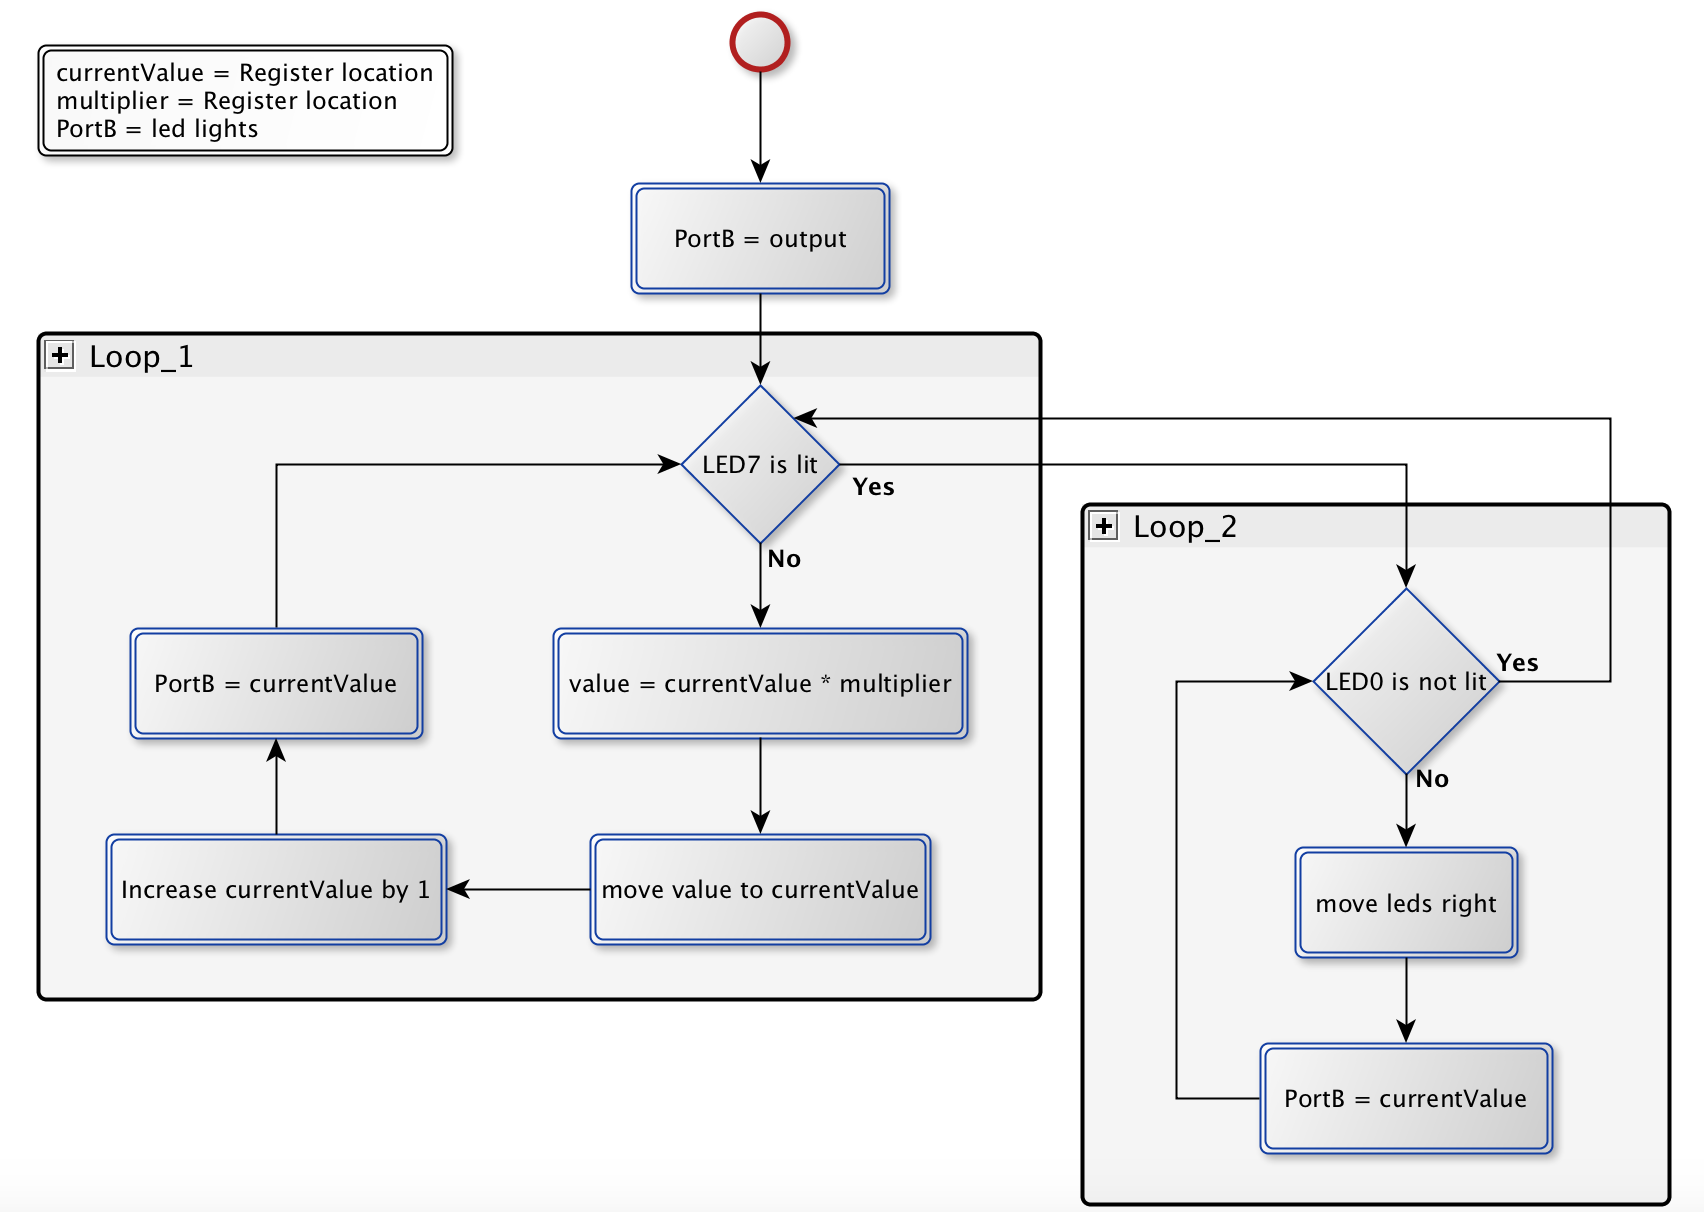
\includegraphics[scale=0.4]{Flowchart_pics/assignment6_pic.png} 
\caption{Flowchart}
\label{}
\end{figure}

\subsection{Method}
We started by trying to figure out the mathematical formula for finding Johnson values. In decimal, the values for an 8-bit Johnson counter are: 0, 1, 3, 7, 15, 31, 63, 127 and 255. We realized that we could get the next value by multiplying by 2 and adding 1, which gives the recurrence relation

\begin{equation*}
    J_n = J_{n-1} \cdot 2 + 1, \qquad n \in \mathbb{N}_0
\end{equation*}

With this we could get both the next and previous Johnson value. In the case of getting the previous value, we considered that we are dealing with integers, which because of truncating means we only needed to divide the current value by 2 to count down the counter.

As with assignment 5, we start by setting the stack pointer since we are going to use a subroutine for the delay function. We also set \texttt{PORTB} as output. To count the Johnson counter up and down, we created two loops: \texttt{count\_up} and \texttt{count\_down}. In \texttt{count\_up} we multiply the current counter value by 2 by shifting it to the left and then increment it by 1 before outputting the value to the LEDs. We repeat this until all the LEDs are lit, upon which executions jumps to \texttt{count\_down}. In this loop, we divide the current counter value by 2 by shifting it to the right and then output the value to the LEDs. This is in turn repeated until all the LEDs are turned off, upon which the execution jumps back to \texttt{count\_up} and the process starts again.

When testing the program on hardware, we had some problems with the pull-up resistor causing the LEDs to output inverse states. We figured the easiest way to solve this was to create a subroutine which gets the complement of the current Johnson value and outputs that to the LEDs.


\subsection{Assembly Program}
\avrasm{../src/a6.asm}{}
\end{document}
